\begin{comment}
\end{comment}

\chapter{Comptage variationnel quantique}

%-----------------------------------------------------------------------------%

\subsection*{Plan}

\begin{enumerate}
    \item Expliquer que cette section ne concerne que GM-QAOA
\end{enumerate}

%-----------------------------------------------------------------------------%

\section{Auto-réductibilité des algorithmes variationnels quantiques}

\subsection*{Plan}

\begin{enumerate}
    \item Faire la preuve de l'auto-réductibilité des algorithmes variationnels quantiques
\end{enumerate}

\subsection*{Références}

%-----------------------------------------------------------------------------%

\section{Algorithme VQCount}

\subsection*{Plan}

\begin{enumerate}
    \item Vulgariser l'algorithme de manière général
    \item Expliquer rigoureusement l'algorithme
    \item Faire le lien entre la notation utilisée dans les algorithmes de comptage classique
    \item Faire la comparaison avec les travaux précédents
    \item Rajouter l'algorithme complet en pseudo-code
\end{enumerate}

\subsection*{Références}

\definecolor{myblue}{rgb}{0.33725490196078434, 0.7558823529411766, 0.9137254901960784}
\definecolor{myred}{rgb}{0.8666666666666667, 0.3607843137254902, 0.3607843137254902}
\definecolor{mysilver}{rgb}{0.7529411764755882, 0.7529411764755882, 0.7529411764755882}
\definecolor{myyellow}{rgb}{0.9411764705882353, 0.8941176470588236, 0.25882352941176473}
\definecolor{mygreen}{rgb}{0.0, 0.6196078431372549, 0.4509803921568627}
\definecolor{mypink}{rgb}{0.8, 0.47450980392156855, 0.6549019607843136}
\definecolor{mybluedark}{rgb}{0.0, 0.44705882352941173, 0.6980392156862745}
\definecolor{myorange}{rgb}{0.9019607843137255, 0.6235294117647059, 0.0}
\definecolor{myviolet}{rgb}{0.3254901960784314, 0.1450980392156863, 0.4980392156862745}


% \begin{figure}[t]
%     \centering
%     \begin{quantikz}[font=\sffamily]
%       \ket{0} & \gate[style={fill=mysilver!85}][0.80cm]{H} & \gate[wires=4, nwires=3, style={fill=myblue!85}][1.30cm]{U_P (\alpha)} & \gate[wires=4, nwires=3, style={fill=myred!85}][1.30cm]{U_D (\beta)} & \ \ldots\ \qw & \gate[wires=4, nwires=3, style={fill=myblue!85}][1.30cm]{U_P (\alpha)} & \gate[wires=4, nwires=3, style={fill=myred!85}][1.30cm]{U_D (\beta)} & \qw \\
%       \ket{0} & \gate[style={fill=mysilver!85}][0.80cm]{H} & & & \ \ldots\ \qw & & & \qw \\
%       \vdots & & & & & & & \\
%       \ket{0} & \gate[style={fill=mysilver!85}][0.80cm]{H} & & & \ \ldots\ \qw & & & \qw
%     \end{quantikz}
%     \caption{}
% \end{figure}

% \begin{figure}[t]
%     \centering
%     \begin{quantikz}
%       \ket{0} & \gate[style={fill=myyellow!55}][0.80cm]{X^{c}} & \gate[wires=4, nwires=3, style={fill=myblue!85}][1.30cm]{U_P (\alpha)} & \qw & \ \ldots\ \qw & \gate[wires=4, nwires=3, style={fill=myblue!85}][1.30cm]{U_P (\alpha) } & \qw & \qw \\
%       \ket{0} & \gate[style={fill=mysilver!85}][0.80cm]{H} & & \gate[wires=3, nwires=2, style={fill=myred!85}][1.30cm]{U_D (\beta)} & \ \ldots\ \qw & & \gate[wires=3, nwires=2, style={fill=myred!85}][1.30cm]{U_D (\beta)} & \qw \\
%       \vdots & & & & & & & \\
%       \ket{0} & \gate[style={fill=mysilver!85}][0.80cm]{H} & & & \ \ldots\ \qw & & & \qw
%     \end{quantikz}
%     \caption{}
% \end{figure}

\begin{figure*}[t]
    \centering
    \begin{subfigure}[h]{0.45\textwidth}
    \centering
    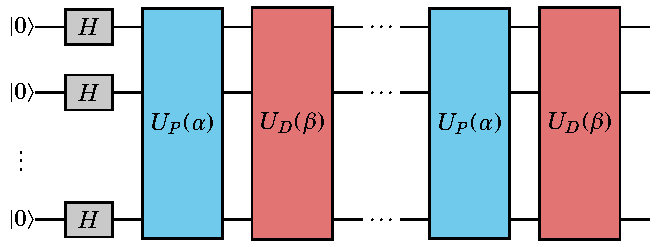
\includegraphics[width=1\textwidth]{figures/qaoa-self-reducibility-1.pdf}
    \caption{}
    \label{fig:quantum-circuit-a}
    \end{subfigure}
    \begin{subfigure}[h]{0.45\textwidth}
    \centering
    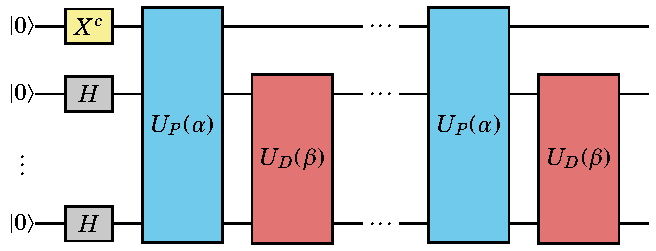
\includegraphics[width=1\textwidth]{figures/qaoa-self-reducibility-2.pdf}
    \caption{}
    \label{fig:quantum-circuit-b}
    \end{subfigure}
\caption{}
\label{fig:quantum-circuit}
\end{figure*}

%-----------------------------------------------------------------------------%

\section{Module VQCount}

\subsection*{Plan}

\begin{enumerate}
    \item Expliquer les librairies python dévelopées
    \item Décrire \textit{qaoa-quimb}
    \item Décrire \textit{VQCount}
\end{enumerate}

\subsection*{Références}